% !TEX root = ../main.tex
\subsubsection{Alignment Effect}
\label{sssec::alignment_effect}
    % Introduction: The problem.
    The RG-F experiment's data is divided based on the season over which runs take place, thus there is Spring 2020 and Summer 2020 data.
    Based on the run group's guidelines, it is recommended to use Summer data, as it has seen more calibration than the Spring data.
    However, this calibration work hasn't included the FMT detector, and a strong misalignment effect is observed.

    % Cause of the problem.
    By simple visual inspection, two peaks can be clearly seen between $z = -36$ cm and $z = -30$ cm in figure \ref{fig::12.41::dc_vs_fmt_vz_11983}.
    These peaks are merged in figure \ref{fig::vz_012933}.
    As discussed in section \ref{12::fmt_alignment_and_reconstruction}, this issue comes from a lack of correction for FMT misalignments.

    % Solution.
    The simplest solution is to use Spring data.
    While more work has been put on Summer data, it mainly pertains to the central detector; unrelated to this analysis.
    Figure \ref{fig::vz_012016} shows the same $v_z$ plot from Spring 2020 run 12016.
    Both peaks are clearly visible in this plot, suggesting that misalignments are properly accounted for in the run.

    \begin{figure}[t!]
        \centering\frame{
        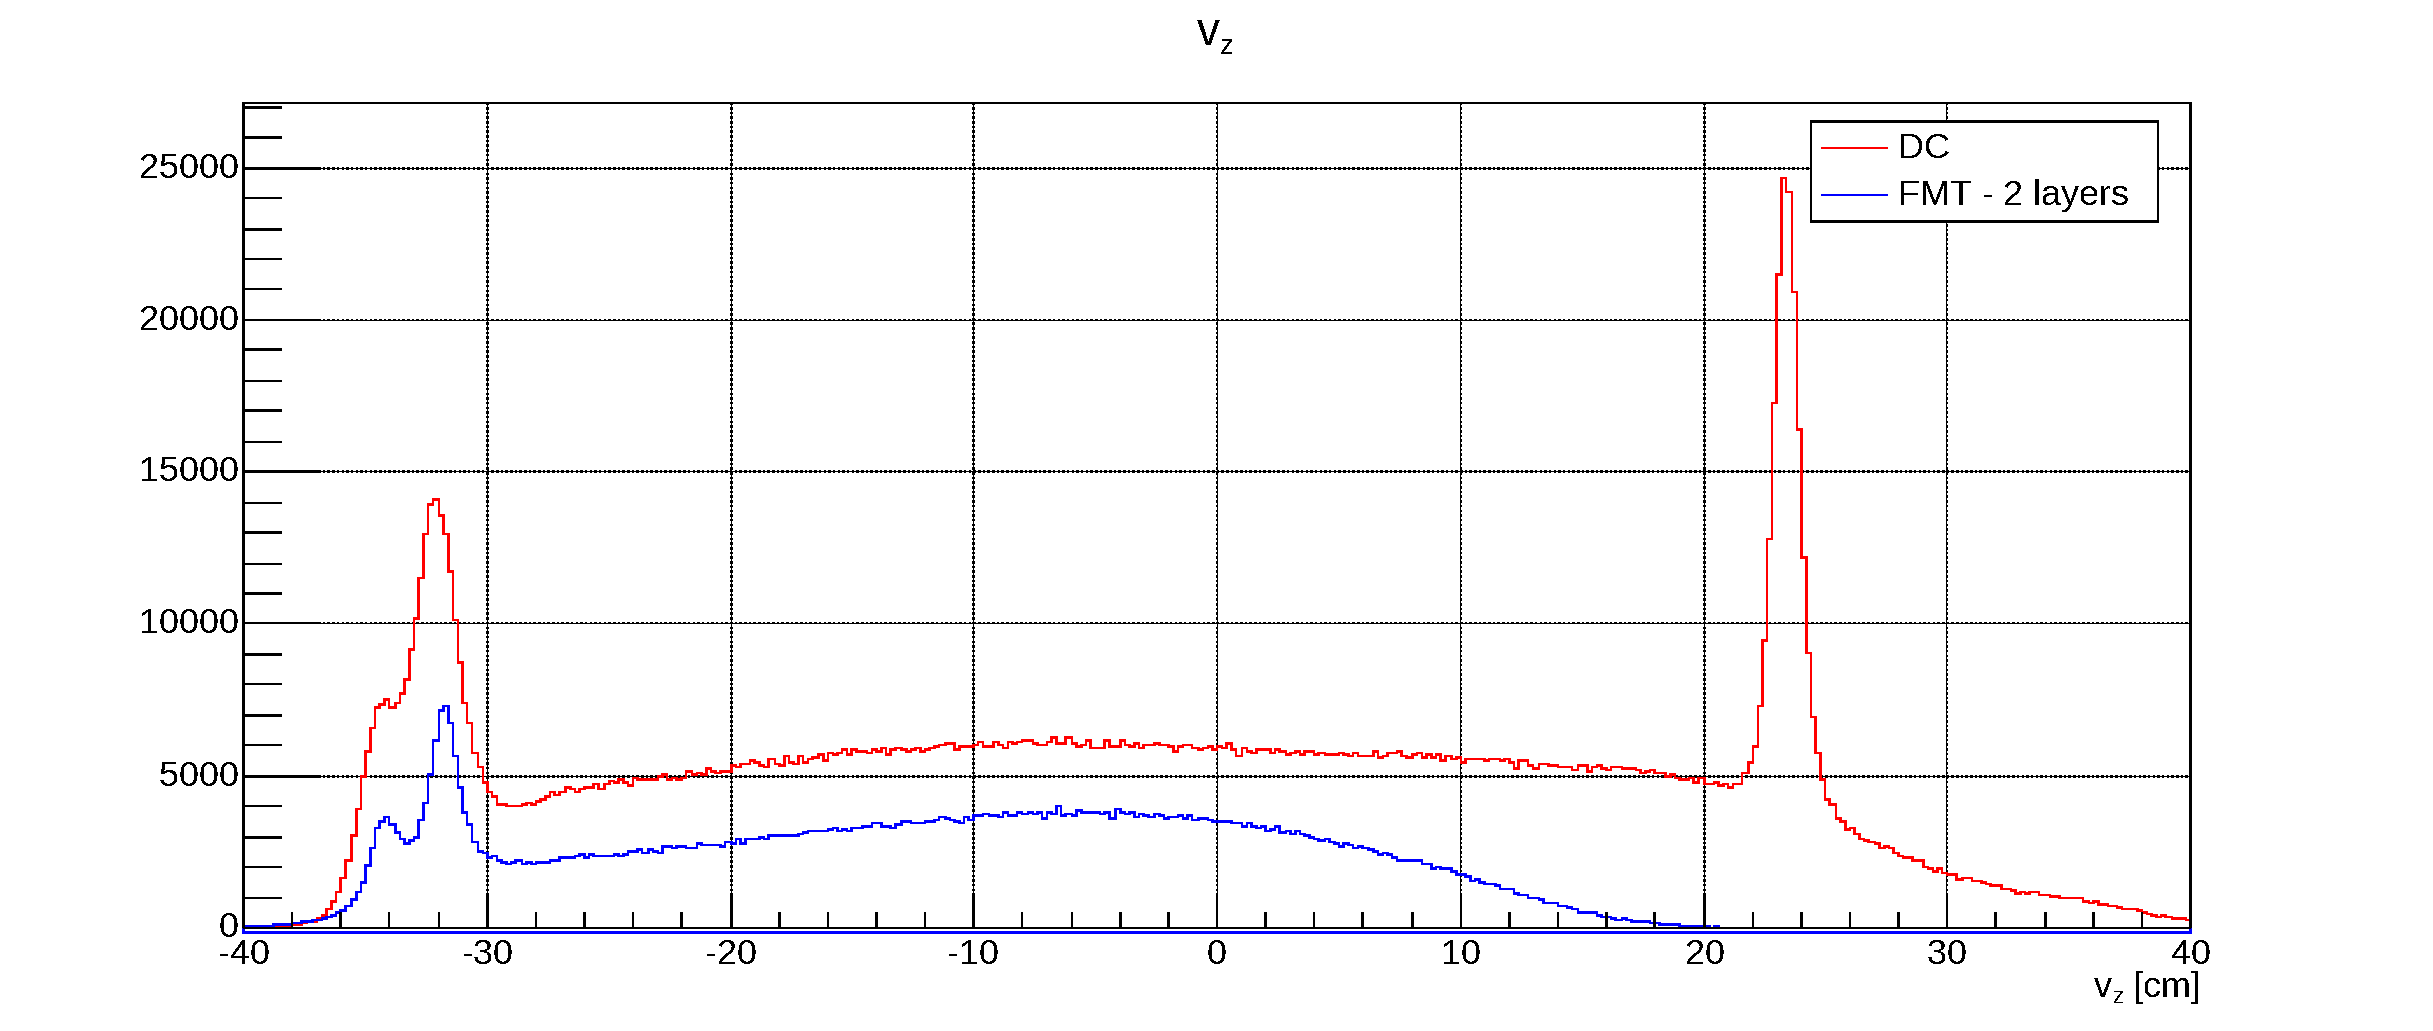
\includegraphics[width=\textwidth]{11vz_012016.pdf}}
        \caption[$v_z$ for DC and FMT, run 12016]{$v_z$ for DC (in red) and FMT (in blue). Spring 2020 data, run 12016. The upstream twin peaks can be clearly distinguished, suggesting a correct misalignment correction.}
        \label{fig::vz_012016}
    \end{figure}
